\documentclass{if-beamer}
\begin{document}
	
	\title[Campus Formoso do Araguaia]{Configuração de Redes e Servidores}
	\subtitle{Aula 0 }
	\author{Gilmar Gomes do Nascimento}
	\institute[IFTO]{
		Instituto Federal do Tocantins\\
		Campus Formoso do Araguaia
	}
	\date{\today}
	\logo{
		
\includegraphics[scale=0.0085]{logo.jpg}
	}
	\subject{Servers} % metadata
	
	\graphicspath{{figuras/}}
	%---------------------------------------------------------------------------------
	\begin{frame}
		\titlepage
	\end{frame}
	
	\begin{frame}{Formação Acadêmica}
	\begin{itemize}
	\item Ciência da Computação - UFT   2009 -- 2014
	\item Especialização Lato Senso - ESAB - 2019
	\item Especialização Lato Senso - Focus - 2021
	\item Mestrado em Ciência da Computação - UTFPR - 2024 - atualmente 
	\end{itemize}
	
	\end{frame}
	
	\begin{frame}{Atuação Profissional}
	\begin{itemize}
	\item Instrutor de Informática  - SENAC - TO  - 2014, 2015
	\item Professor de Informática - Colégio da Polícia Militar - TO - 2015 - 2016
	\item Analista de Suporte -  Justiça Federal  - TO - 2017 
	\item Professor substituto EBTT - IFTO - Campus Colinas do Tocantins - 2017 - 2019
	\item Professor EBTT - IFAM - Campus Boca do Acre - 2021 - 2026
	\item Professor EBTT - IFTO - Campus Formoso do Araguaia - 2026
	\end{itemize}
	\end{frame}
	
	
	\begin{frame}{Ementa}
	\begin{figure}
	\centering
	\includegraphics[scale=0.38]{ementa-servers}
	\end{figure}
	\end{frame}
	
	
	\begin{frame}{DevOps}
	\begin{figure}
	\centering
	\includegraphics[scale=0.48]{devops}
	\end{figure}
	\end{frame}
	
	\begin{frame}{DevOps}
	DevOps é uma cultura e um conjunto de práticas que une as equipes de desenvolvimento de software (Dev) e de operações de TI (Ops). O objetivo é acelerar a entrega de aplicativos com mais segurança, automação e alta qualidade, por meio de ciclos contínuos de testes, testes de integração e monitoramento.
	\end{frame}
	
	\begin{frame}{SysAdmin}
	\begin{figure}
	\centering
	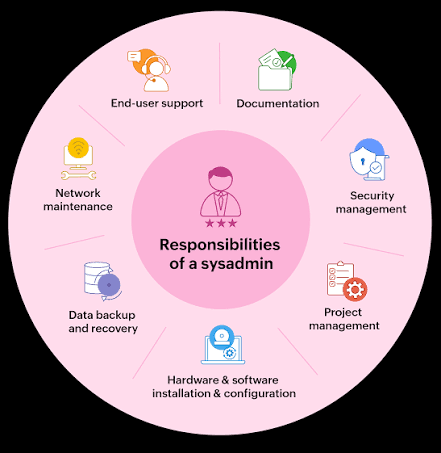
\includegraphics[scale=0.48]{sysadmin}
	\end{figure}
	\end{frame}
	
	\begin{frame}{SysAdmin}
	SysAdmin (Administrador de Sistemas) é o profissional de TI responsável por configurar, gerenciar, manter e garantir a segurança e o funcionamento contínuo de servidores, redes e da infraestrutura de computadores de uma organização.

	\end{frame}
	\begin{frame}{Tipos de servidores}
	\begin{figure}
	\centering
	\includegraphics[scale=0.46]{types-servers}
	\end{figure}
	\end{frame}
	
	\begin{frame}[allowframebreaks]{UTC}
	O UTC (Tempo Universal Coordenado) é o principal padrão de tempo global que define as horas exatas no mundo. Ele se baseia em relógios atômicos e serve de referência para calcular todos os fusos horários, substituindo o antigo horário GMT. 
	Também conhecido como \textbf{tempo civil}, é o fuso horário de referência a partir do qual se calculam todas as outra zonas horárias do mundo.

	\framebreak
	\begin{figure}
	\includegraphics[scale=0.39]{utc}
	\end{figure}
	\end{frame}
	
	\begin{frame}[allowframebreaks]{NTP(Network Time Protocol)}
		O Network Time Protocol (NTP) é amplamente usado para sincronizar um computador a servidores de horário da Internet ou outras fontes, como receptores de rádio ou satélite ou serviços de modem de telefone. 
	\framebreak
	\\ Geralmente, ele fornece precisão menor que um milissegundo em LANs e até alguns milissegundos em WANs. As configurações de NTP típicas utilizam vários servidores redundantes e caminhos de rede para obter uma alta precisão e confiabilidade. 
	\framebreak
	\\ O NTP usa o algoritmo de Marzullo para sincronizar o tempo com a versão atual do NTP. Ele pode manter o tempo na Internet pública em até 10 milissegundos e pode ter um desempenho ainda melhor nas LANs. Os servidores de horário NTP funcionam no conjunto TCP/IP e dependem da porta 123 do Protocolo de Datagrama do Usuário (UDP - User Datagram Protocol).\\
	\framebreak
	O algoritmo NTP usa essa referência de tempo para determinar a quantidade para adiantar ou retardar o relógio do sistema ou da rede. O NTP analisa os valores de timestamp e a frequência dos erros e sua estabilidade. Um servidor NTP mantém uma estimativa da qualidade dos relógios de referência e de si mesmo.\\
	\begin{figure}
	\includegraphics[scale=.4]{architecture-ntp}
	\end{figure}
	
	\end{frame}
	
\begin{frame}[allowframebreaks]{NTP.BR}
\begin{figure}
\includegraphics[scale=.45]{ntp-br}
\caption{Arquitetura NTP}
\end{figure}
\framebreak
A iniciativa NTP.br tem por objetivo oferecer condições para que os servidores Internet no Brasil estejam sincronizados com a hora certa. Mais especificamente, com a Hora Legal Brasileira. Para isso foi firmado um acordo entre o Observatório Nacional (ON), que é a entidade legalmente responsável pela definição do padrão de tempo nacional, a Hora Legal Brasileira, e o NIC.br. \\

\framebreak
O ON tem como atribuição legal a geração, conservação e disseminação da Hora Legal Brasileira. Rastreado ao Bureau International des Poids et Mesures (BIPM), na França, participa do Tempo Universal Coordenado (TUC ou UTC), juntamente com os órgãos disseminadores de tempo e frequência dos demais países. \\
\framebreak
Pelos termos do acordo o ON disponibiliza, sem qualquer ônus, ao Núcleo de Informação e Coordenação do Ponto BR – NIC.br, o sincronismo à Hora Legal Brasileira, seguro, confiável, rastreável e auditável, e o NIC.br disponibiliza, sem qualquer ônus, ao ON um conjunto de equipamentos necessários à manutenção da infra-estrutura de sincronismo. \\
\framebreak
\begin{figure}
\includegraphics[scale=0.5]{cesio}
\end{figure}
\end{frame}


\begin{frame}{Pools}
\begin{figure}
\includegraphics[scale=.35]{pools}
\end{figure}

\end{frame}
\begin{frame}{Hora certa}
\begin{figure}
\includegraphics[scale=0.8]{syncro-time}
\end{figure}
\end{frame}	

\begin{frame}{Configurando no MS Windows}
\begin{figure}
\includegraphics[scale=0.37]{setting-time}
\end{figure}
\end{frame}

\begin{frame}[allowframebreaks]{Atenção}
Não se recomenda a utilização de dispositivos com sistema operacional Windows como servidores de tempo, com exceção do uso de servidores domain controller no Active Directory, que sincroniza automaticamente os demais dispositivos no mesmo domínio. Não se recomenda a instalação da implementação de referência do NTP, disponível em ntp.org, ou de outros softwares para as funções de cliente ou servidor NTP em dispositivos utilizando Windows 
\framebreak

\textbf{Não é possível sincronizar o NTP com o serviço de tempo baseado em W32}

Quando os roteadores Cisco são configurados para usar os servidores NTP colocados no Ative Diretory, os roteadores Cisco não recebem nenhum pacote NTP do servidor NTP. Esse problema ocorre porque os roteadores Cisco usam os domínios NTP e Ative Diretory usam o serviço W32Time.\\

\framebreak
A W32Time usa o Simple Network Time Protocol (SNTP), um subconjunto do NTP, para sincronização de tempo. O SNTP e o NTP usam o mesmo formato de pacote de rede. A principal diferença entre o SNTP e o NTP é que o SNTP não fornece as funções de verificação de erros e filtragem fornecidas pelo NTP. Os roteadores e switches da Cisco usam o NTP e permitem todas as funções de verificação de erros e filtragem fornecidas pelo NTP v3. \\

\framebreak

O Windows W32Time mostra que é uma implementação de SNTP interna (em vez de se afirmar como NTP). O Cisco IOS-NTP, que tenta sincronizar com o W32Time, obtém seu próprio valor de dispersão de raiz que envia ao W32Time e isso se revela caro para que o Cisco IOS-NTP sincronize. Como o valor de dispersão raiz do Cisco IOS-NTP vai além de 1000 ms, ele se dessincroniza (procedimento de seleção de tempo). \\

\framebreak
Para contornar esse problema e sincronizar um roteador baseado no Cisco IOS, use um servidor NTP autoritativo na Internet, uma caixa UNIX que execute NTPD ou um GPS em determinadas plataformas. \\
\end{frame}
	
	\begin{frame}{Não sincronização com servidores de horário público}
		\begin{itemize}
		  \item Listas de controle de acesso que não permitem a passagem de pacotes da porta 123 UDP
		\item Configuração incorreta nos roteadores, como os comandos clock timezone e clock Summer-time estão ausentes nos roteadores
		\item O servidor de tempo público está inoperante
		\item O software do servidor NTP em NT ou UNIX está mal configurado
		\item Mais tráfego está no roteador e mais tráfego no caminho para o servidor
		\item O mestre NTP perdeu a sincronização e o roteador perde a sincronização periodicamente
		\item Alto uso de CPU
				\end{itemize}
		
	\end{frame}
	\begin{frame}{Problemas envolvendo horário}
				
		\begin{block}{}
			\begin{itemize}
			\item Sistemas de arquivos (data de criação/modificação de arquivos(timestamp))
			\item Agendadores de eventos(cron)
			\item Autenticação
			\item Investigação de incidentes
			\end{itemize}
		\end{block}
	\end{frame}
	
	\begin{frame}
	\begin{block}{Atividade}
	No que diz a respeito ao NTP do conjunto de protocolos TCP/IP, é correto afirmar que pertence à camada de

	
	\begin{enumerate}
		\item Aplicação e se destina à transferência de notícias para os computadores da rede
		\item Aplicação e se destina à sincronização dos relógios dos equipamentos conectados na rede
		\item Rede e se destina à sincronização do timestamp dos pacotes transportados na rede
		\item Rede e se destina ao envio de notícias e informações entre os roteadores da rede
		\item Transporte e se destina ao envio, em tempo real, dos pacotes de dados de chats
	
	\end{enumerate}
	
	\end{block}
	\end{frame}
	\begin{frame}[allowframebreaks]{NTS}
	O NTS (Network Time Security) é uma extensão de segurança do NTP. Ele fornece mecanismos para autenticar e criptografar mensagens NTP, garantindo que os dados de horário recebidos sejam seguros e autênticos. O NTS foi projetado para compatibilidade retroativa com a infraestrutura NTP existente. Isso permite a implantação gradual sem exigir mudanças nos servidores NTP existentes que não suportam NTS. 
	\framebreak
	\begin{itemize}
		\item Identidade: usa a estrutura de chaves públicas X.509
		\item Autenticação: verifica criptograficamente que a informação de relógio nos
pacotes NTP é autêntica, produzida por um servidor identificável.
\item Proteção contra ataques de repetição: o cliente pode detectar
\item Consistência entre requisições e respostas: o cliente pode verificar
\end{itemize}
\framebreak
\begin{itemize}
\item Privacidade: NTS não vaza nenhuma informação que permitiria a um terceiro
determinar que dois pacotes vindos de redes diferentes se originaram no mesmo
cliente
\item Não amplificação: as respostas nunca são maiores do que as requisições
\item Escalabilidade: os servidores não guardam estado dos clientes, então podem
servir a um grande número
\item Desempenho: o NTS não degrada a qualidade da sincronização dos relógios
\end{itemize}
	\end{frame}
	
\begin{frame}[allowframebreaks]{NTP e Segurança}
	Segurança não era uma preocupação na correta sincronização dos relógios no passado
	\begin{block}{Mas muita coisa mudou}
		\begin{itemize}
			\item a Internet cresceu e se descentralizou
			\item há muitas evidências de um tratamento inadequado da segurança no NTP
			\item há um interdependência crescente entre o registro do tempo e a segurança
			\item há requisitos legais e de conformidade
		\end{itemize}
	\end{block}
	\framebreak
\begin{itemize}	
	\item Falhas no software ou na configuração
	\item o ntpd é um dinossauro, gigante, com suporte a uma miríade de hardwares e sistemas, as opções padrão não são as mais seguras
	\item Falhas no protocolo
	\item Falta de mecanismos adequados de segurança
\end{itemize}
\end{frame}


\begin{frame}{Certificados TLS}
O TLS é usado para estabelecer conexões seguras e autenticadas na Internet
\begin{block}{heartbleed}
 Se um ataque NTP conseguir fazer um cliente voltar no tempo, ele pode aceitar certificados fraudados. Por exemplo certificados emitidos antes de 2014 com a falha do heartbleed.
\end{block}
\end{frame}

\begin{frame}{DNSSEC}
O DNSSEC provê autenticação para o sistema de nomes. 
\begin{block}{atacado}
Se um resolver está configurado pra fazer ``strict validation", ou seja, não responde se as queries falham a validação do DNSSEC, então um ataque NTP que leva o resolver para frente no tempo pode fazer com que todos os certificados e chaves expirem. Um ataque NTP que leve para o passado pode permitir ataques de repetição.
\end{block}

\end{frame}

\begin{frame}{Instalação e configuração do servidor}
\begin{itemize}
\item chrony
\item ntpsec
\item openntpd
\end{itemize}

\end{frame}
	
	
	\begin{frame}[allowframebreaks]{Referências Bibliográficas}
		\bibitem{noauthor_undated-xq}
NTP.br. \url{https://ntp.br/conteudo/ntp/}. Acessado em: 6 de agosto de 2026.

\bibitem{Cisco_System_Inc2022-gp}
Cisco System, Inc. (2022). Identificar e Solucionar Problemas do Network Time Protocol (NTP). 26 de setembro de 2022.

\bibitem{ibm}
IBM. (2025). Tivoli Application Dependency Discovery Manager. \url{https://www.ibm.com/docs/pt-br/taddm/7.3.0?topic=problems-synchronization-server}. Acessado em: 6 de agosto de 2026.

\bibitem{cisco}
Cisco. (2025). Use as práticas recomendadas para o Network Time Protocol. \url{https://www.cisco.com/c/pt_br/support/docs/availability/high-availability/19643-ntpm.html}. Acessado em: 6 de agosto de 2026.

\bibitem{suse}
SUSE. (2026). Sincronizando o horário por meio de NTP/NTS. \url{https://documentation.suse.com/pt-br/sle-micro/6.1/html/Micro-ntp-time-synchronization/index.html}. Acessado em: 6 de agosto de 2026.

\bibitem{Moreiras2021}
Moreiras, Antonio Marcos. (2021). NTP e NTS de Forma Correta e Segura, Sincronismo de Tempo na Internet. Nic.br. \url{https://bibliotecadigital.acervo.nic.br/server/api/core/bitstreams/129d1169-25b5-49ce-b015-28ffadc440da/content}. Acessado em: 6 de agosto de 2026.
	\end{frame}	
	
\end{document}
